\documentclass{article}
\usepackage[utf8]{inputenc}
\usepackage[noend]{algorithmic}
\usepackage{amsmath}
\usepackage{graphics}
\usepackage{graphicx}
\usepackage{float}

\textwidth              16 cm
\textheight             24.5  cm
\oddsidemargin          -1   cm
\evensidemargin         -1cm
\topmargin              -1 cm

\title{Grafuri Tema 1}
\author{Oancea Ionut Eugen 3A5, Marius Dinu 3A5}
\date{November 2020}

\begin{document}

\maketitle

{\bf 1.}
\begin{algorithmic}
\STATE rezolvare(G=(V,E), k)
\IF{(k $>$ $\lvert$ V $\rvert$)} 
    \RETURN "Nu"; //nu se pot crea destule partitii nici macar daca fiecare are cate un nod
\ENDIF
\STATE nrConexe $\gets$ 0;
\FOR{(x din V)}
    \IF{(viz[x] == 0)} 
        \STATE BFS(x); //retin ce noduri au fost vizitate atunci cand fac BFS
        \STATE nrConexe++;
    \ENDIF
\ENDFOR

\IF{(nrConexe $\leq$ k)}
    \RETURN "Da";
\ELSE
    \RETURN "Nu";
\ENDIF
\end{algorithmic}
\vspace{0.5cm}

Explicatie: Numar cate componente conexe are graful. Daca sunt mai putin de k componente, le pot imparti in oricate componente conexe mai mici, deci raspunsul este afirmativ. Daca nu, partitionand graful nu pot "uni" componente conexe, deci este imposibil sa reduc numarul lor pentru a obtine k componente.

\vspace{0.5cm}

{\bf 2.} {\bf a.} Diametrul este 2 deoarece intre oricare 2 noduri alese din graf exista un drum de lungime 2 (drumul care trece prin vecinul lor comun). Daca graful ar contine un circuit de lungime 4, atunci nodurile din acesta ar avea mai mult de un vecin comun (ar avea cate 2). Deci, este imposibil. 
\begin{figure}[H]
\centering
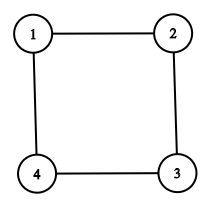
\includegraphics[scale=0.5]{graph1.png}
\caption{fiecare nod are cate 2 vecini comuni - ex.: 1 si 3 ii au pe 2 si 4}
\end{figure}

{\bf b.} Conform cerintei, oricare 2 noduri au 1 vecin comun. Daca acele 2 noduri sunt vecine, inseamna ca exista muchii atat intre ele cat si intre ele si vecinul lor comun. Deci, se formeaza o 3-clica. Conform demonstratiei anterioare, fiecare nod este intr-o 3-clica impreuna cu orice vecin de-al sau. Deoarece toate nodurile din 3-clica sunt vecine, putem extinde demonstratia si afirma ca fiecare 2 vecini de-ai unui nod formeaza cu acesta o 3-clica. Alegem un nod la intamplare, v. v are d(v) vecini, iar conform demonstratiei anterioare, impreuna cu cate 2 dintre acestia formeaza 3-clici. Deci, in subgraful indus de v si vecinii sai se formeaza d$_G$(v)/2 3-clici. Fiecare 3-clica are 3 muchii, deci numarul de muchii este 3d$_G$(v)/2.

{\bf c.} Alegem 2 noduri neadiacente la intamplare. Din cerinta reiese ca cele 2 noduri au un vecin comun, si din {\bf b} reiese ca fiecare dintre cele 2 perechi de vecini fac parte din cate o 3-clica (nu pot fi toate 3 in aceeasi clica pentru ca ar trebui ca nodurile alese neadiacente sa fie vecine). Deci, cele 2 noduri alese aleator au cate 2 vecini fiecare (cel comun si vecinul din clica al fiecaruia).

{\bf 3.}{\bf a.}
\begin{algorithmic}
\STATE rezolvare(G=(V,E), altitudini[])
\vspace{0.1cm}
\STATE costuriDus[i] $\gets$ costuriIntors[i] = -1, i=$\overline{1, n}$; //initializez costurile pentru parcurgerile din ambele sensuri
\STATE costuriDus[x] $\gets$ costuriIntors[y] = 0; //x este nodul de unde pornesc, y este nodul unde vreau sa ajung
\STATE costFinal $\gets \infty$;
\STATE DFS\_dus(G, altitudini, x, costuriDus);
\STATE DFS\_intors(G, altitudini, y, costuriDus, costuriIntors, costFinal);
\RETURN costFinal;

\vspace{0.8cm}

\STATE DFS\_dus(G, altitudini[], start, costuriDus[])
\vspace{0.1cm}
\FOR{(x din V)}
    \IF{(altitudini[x] $>$ altitudini[start] \&\& costuriDus[x] == -1)}
    \STATE costuriDus[x] $\gets$ costuriDus[start] + $\alpha$(start,x);
    \STATE DFS\_dus(G, altitudini, x, costuriDus);
    \ENDIF
\ENDFOR

\vspace{0.8cm}

\STATE DFS\_intors(G, altitudini[], start, costuriDus[], costuriIntors[], costFinal)
\vspace{0.1cm}
\FOR{(x din V)}
    \IF{(altitudini[x] $>$ altitudini[start] \&\& costuriIntors[x] == -1)}
        \STATE costuriIntors[x] $\gets$ costuriIntors[start] + $\alpha$(start,x);
        \IF{(costuriDus[x] $>$ -1)}
            \IF{(costFinal $>$ costuriDus[x] + costuriIntors[x])}
            \STATE costFinal $\gets$ costuriDus[x] + costuriIntors[x]
            \ENDIF
        \ENDIF
        \STATE DFS\_intors(G, altitudini, x, costuriDus, costuriIntors, costFinal);
    \ENDIF
\ENDFOR
\end{algorithmic}
\vspace{1cm}
Explicatie: Deoarece pentru a parcurge un ciclu, studentul ar trebui sa urce, apoi sa coboare (pana in nodul de start al ciclului), iar apoi sa urce din nou (pe traseul ciclului), ceea ce este imposibil deoarece dupa ce a coborat nu mai poate urca, se poate afirma ca graful practic este aciclic. Datorita acestei proprietati, o parcurgere DFS a acestuia dintr-un nod va putea calcula costurile minime pana in celelalte noduri. Fac un DFS din nodul de start spre final, apoi un DFS din nodul final spre start. Primul DFS va salva costurile minime din start pana unde se poate ajunge doar urcand, iar al doilea DFS va salva costurile minime de la final la toate nodurile unde se poate ajunge urcand (practic, costurile minime din orice nod din care se poate ajunge pana la final doar coborand). Costul minim al drumului total va fi costul minim al unei parcurgeri din start pana intr-un nod (urcand) si din acel nod pana la final (coborand). Deci, in implementarea mea, costul minim va fi minimul costurilor totale pana in si din nodurile care apar in ambele parcurgeri (acele noduri sunt posibilele varfuri ale traseului studentului). Complexitatea implementarii este $O(n+m)$ deoarece aceasta este complexitatea fiecarei pargurgeri DFS.

{\bf b.} Acum, graful poate avea cicluri (noduri consecutive la aceeasi inaltime), deci nu mai exista garantia ca DFS sa calculeze costul minim. Astfel, cea mai eficienta solutie ar fi folosirea algoritmului lui Dijkstra (este posibila deoarece nu exista muchii de cost negativ), care are complexitatea $O(m+nlogn)$ (conform cursului 4).

\vspace{0.5cm}

{\bf 4.} {\bf a.} s si u sunt in acelasi subarbore ($T_s^1$) in G - e, deci stergerea muchiei e nu influenteaza drumul de la s la u. Drumul minim de la s la u in G va exista si in G - e, deci cele doua drumuri sunt aceleasi si evident au acelasi cost.

{\bf b.} Conform criteriului de selectie, v si t se afla in acelasi subarbore ($T_s^2$). Deci, exista un drum de la s la t care trece prin $x_2$ (radacina subarborelui). De asemenea, este garantat ca drumul de la $x_2$ la t (sau la s) nu trece prin e (dupa modul cum a fost construit arborele). Deci, exista un drum de la s la t care nu trece prin e care are cost mai mic decat unul care ar trece prin e. Astfel, eliminarea muchiei e nu va influenta drumul de cost minim dintre v si t - acesta va ramane neschimbat in G si in G - e.

{\bf c.} Presupunem prin absurd ca exista un drum de cost minim de la s la t care trece prin mai multe muchii din F. Fie uv ultima dintre aceste muchii (din F) prin care duce drumul. Deoarece drumul selectat de mine este de cost minim, inseamna ca si d(s, u) este de cost minim. Dar, conform constructiei arborelui $T_s$, drumul de cost minim de la s la u (ambele fiind in A) nu trece prin nicio muchie din F (altfel ar fi si acestea in A). Deci, am ajuns la contradictie. Drumul de cost minim contine doar o muchie din F.

{\bf d.} Conform {\bf c}, drumul minim contine doar o muchie din F. Fie aceasta muchie uv. Conform {\bf a} si {\bf b}, costurile minime ale drumurilor din s in u si din v in t in G sunt aceleasi cu cele din G - e. Deci, proprietatea este demonstrata.

{\bf e.} Cum graful are muchii cu costuri strict pozitive, putem aplica algoritmul lui Dijkstra pornind din s. Conform cursului 4, acest algoritm are complexitatea $O(m + nlogn)$.

\end{document}

